%        File: coupling_outline.tex
%     Created: Friday March 4 12:24:15 2011
% Last Change: Friday March 4 12:24:20 2011
%
\documentclass[letterpaper]{article}
\usepackage[top=1.0in,bottom=1.0in,left=1.0in,right=1.0in]{geometry}
\usepackage{appendix}
\usepackage{verbatim}
\usepackage{amssymb}
\usepackage{graphicx}
\usepackage{longtable}
\usepackage{amsfonts}
\usepackage{amsmath}
\usepackage[usenames]{color}
\usepackage[
naturalnames = true, 
colorlinks = true, 
linkcolor = black,
anchorcolor = black,
citecolor = black,
menucolor = black,
urlcolor = blue
]{hyperref}
\usepackage{listings}
\usepackage{textcomp}
\definecolor{listinggray}{gray}{0.9}
\definecolor{lbcolor}{rgb}{0.9,0.9,0.9}
\lstset{
  backgroundcolor=\color{lbcolor},
  tabsize=4,
  rulecolor=,
  language=c++,
        basicstyle=\scriptsize,
        upquote=true,
        aboveskip={1.5\baselineskip},
        columns=fixed,
        showstringspaces=false,
        extendedchars=true,
        breaklines=true,
        prebreak =
        \raisebox{0ex}[0ex][0ex]{\ensuremath{\hookleftarrow}},
        frame=single,
        showtabs=false,
        showspaces=false,
        showstringspaces=false,
        identifierstyle=\ttfamily,
        keywordstyle=\color[rgb]{0,0,1},
        commentstyle=\color[rgb]{0.133,0.545,0.133},
        stringstyle=\color[rgb]{0.627,0.126,0.941},
}

\author{Stuart R. Slattery
\\ \href{mailto:sslattery@wisc.edu}{\texttt{sslattery@wisc.edu}}
}

\date{Wednesday, October 12 2011}
\title{Outline of the Coupling Package}
\begin{document}
\maketitle

\section{Introduction}
For most multiphysics simulations, some form of data transfer between
physics codes is required. In general, data transfer can be performed
through an ad-hoc coupling of the codes with custom software designed
for the specific simulation. However, it is useful to consider a
common framework and an associated interface for data transfer
operations. This common interface, to be fulfilled by each code that
desires to participate in coupling under this framework, should reduce
repeated effort and define generic and reusable software that can be
applied to many forms of multiphysics simulation.

The coupling package aims to define such an interface for coupling in
addition to providing concrete implementations of algorithms and
communication patterns for parallel data transfer using the
information acquired through this interface. This document discusses
the design requirements that will shape this interface along with the
implementation of fundamental transfer algorithms in a simple example.
It should not be the aim of the coupling package to eliminate other
forms of multiphysics data transfer. Rather, it should attempt to
define a useful interface that provides value by simplifying the
coupling process and reducing the barrier of entry for a physics code
to participate in coupling. 

\section{Design Requirements for the Coupling Package}
The coupling package should fulfill the follwing design
requirements:

\begin{itemize}
\item Be able to couple multiple codes that have implemented the
  interface.
\item Be independent of the underlying data structures of the physics
  codes using the interface.
\item Be aware of the potential mesh entity structures that are
  associated with the fields being transferred (i.e. vertices, faces,
  elements, etc.) in the case of multi-dimensional transfers.
\item Be aware of the parallel communication objects that operate the
  codes being coupled.
\item Be able to generate a parallel topology map using information
  made available through the interface.
\item Be able to transfer multiple fields using the topology map and
  information made available through the interface.
\end{itemize}

\section{Preliminary Design of the Coupling Package}

\subsection{Coupling Package Interface}
As part of the requirements listed in the previous section, it is
necessary to define an interface for the coupling package that will
allow access to information held by each physics code being coupled in
order to meet the coupling algorithm requirements in concrete data
transfer implementations.

In its current form, the interface to the coupling package exists as
an abstract interface contained by the Transfer\_Evaluator class. This
interface should be fulfilled by each physics code that desires to
participate in coupling under this framework by creating its own
implementation of the Transfer\_Evaluator. By implementing a transfer
evaluator, a code will provide the necessary information to implement
coupling algorithms.

\subsection{Coupling Package Map}
The topology map for parallel transfer of a field (or potentially a
portion of the field) is stored in the Transfer\_Map class. Although
this class is initially presented as a concrete implementation, in the
future the Transfer\_Map should instead represent an interface for
many forms of mapping corresponding to many forms of coupling
(e.g. point to volume or surface to surface couplings).

\subsection{Coupling Package Manager}
The coupling problem is managed by the Data\_Transfer\_Manager
class. This class is aware of the Transfer\_Evaluator implementations
for each code being coupled as well as topology maps for each type of 
transfer being performed. The Data\_Transfer\_Manager should
ultimately drive how various coupling and transfer algorithms interact
with the physics codes through the Transfer\_Evaluator and the mapping
through the Transfer\_Map. 

\section{Simple Example}
A simple mesh based data transfer example was constructed as a
means of both demonstrating and developing capability for the coupling
package. In terms of the coupling package description presented in the
previous section, this example can be represented by the following
class diagram presented in Fig.\ref{fig:example_domain}. Here, the
coupling package contains the transfer evaluator interface, the
transfer map, and the data transfer manager. In the example package,
codes A and B along with their implementations of the transfer
evaluator can be found. The only link between the coupling package and
the example package is the implementation of the transfer evaluator
interface by each code. 

\begin{figure}[htpb!]
  \begin{center}
    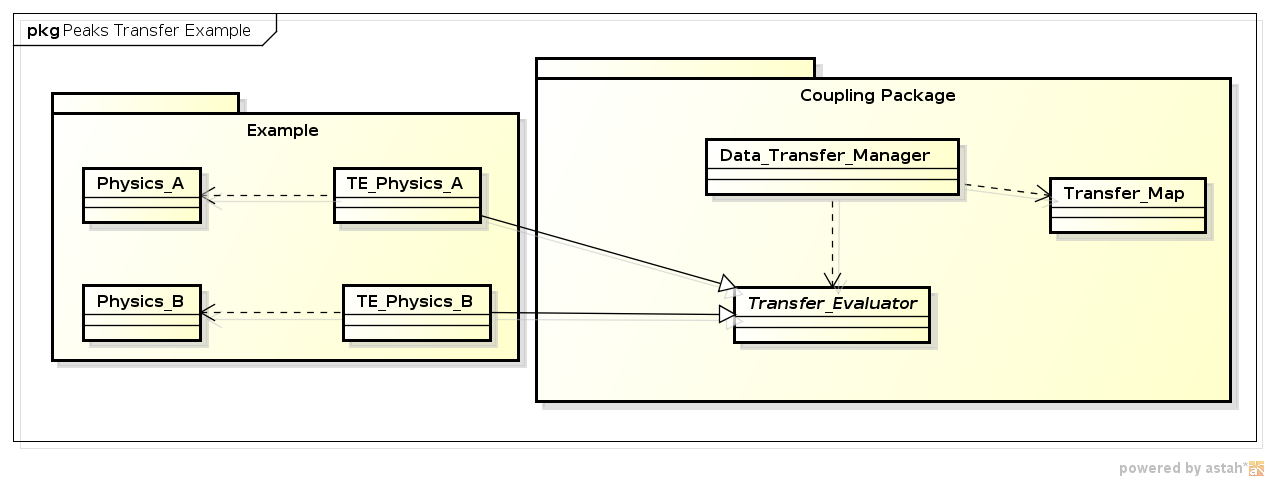
\includegraphics[width=6in]{images/Example_Diagram.png}
  \end{center}
  \caption{\small \sl Class diagram for the simple peaks transfer
    example. The coupling package contains the core classes while the
    example contains codes A and B and their implementations of the
    transfer evaluator.}
  \label{fig:example_domain}
\end{figure}

In this example, code A populates a solution vector with the
peaks function on a fine quad mesh at the center of its mesh cells
with a solve method. Fig.\ref{fig:sol_A} gives the code A mesh and its 
solution. After the solve, the coupling package transfers the solution
from code A to the appropriate data vector associated with the code B
coarse mesh vertices.

\begin{figure}[htpb!]
  \begin{center}
    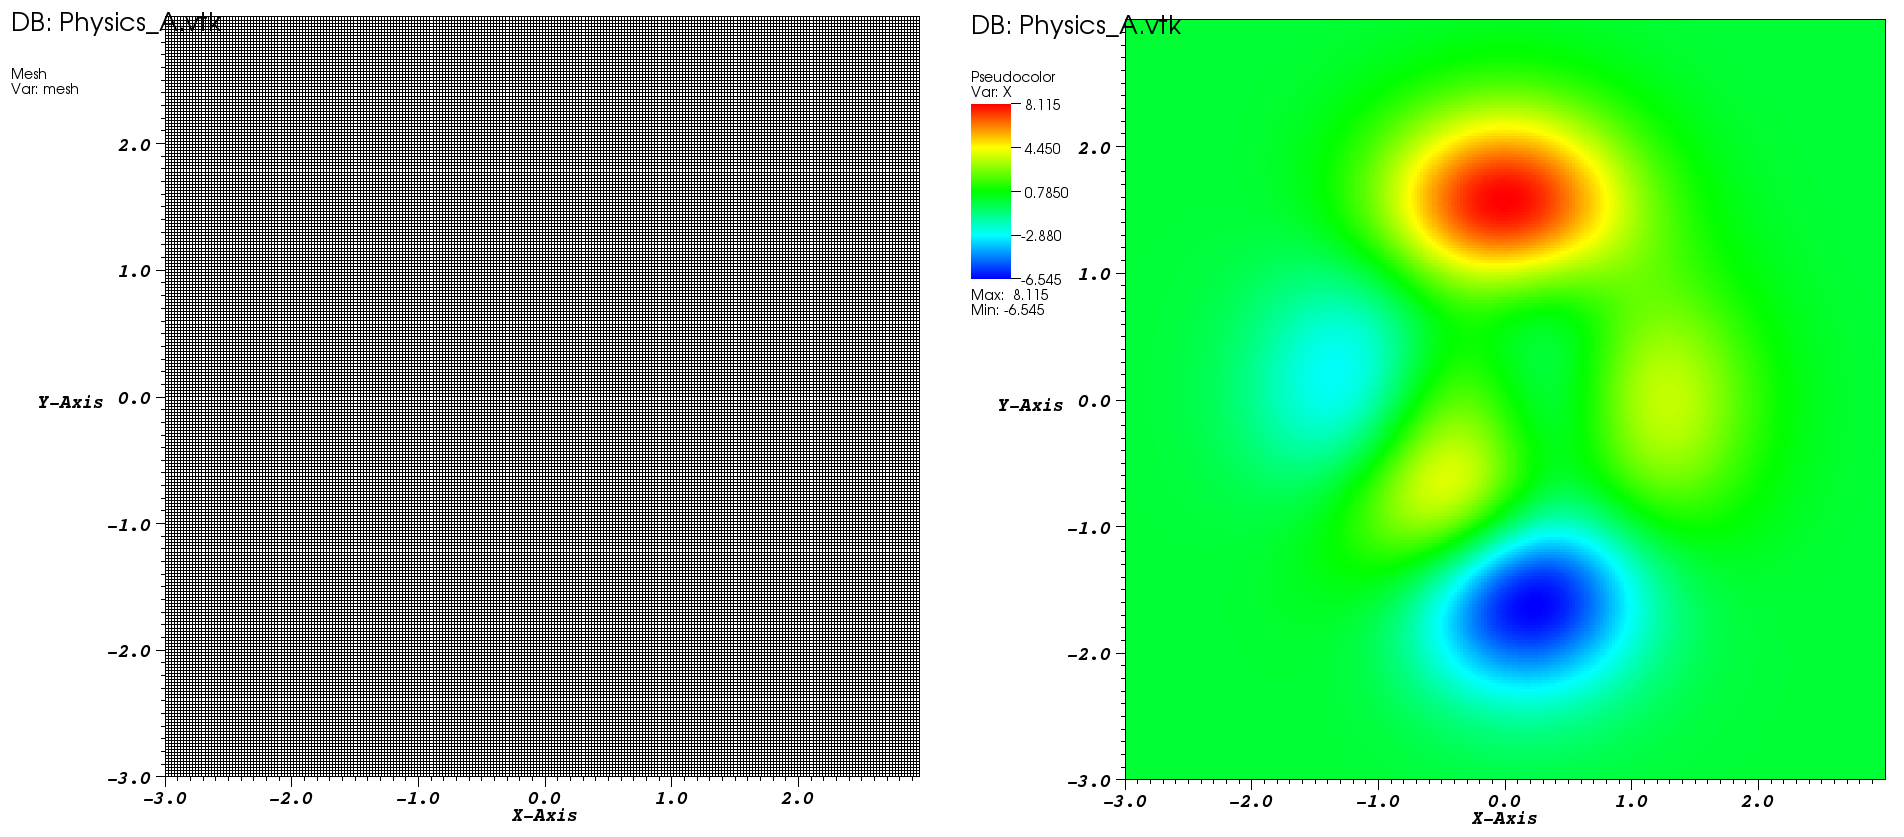
\includegraphics[width=6in]{images/sol_A.png}
  \end{center}
  \caption{\small \sl Fine quad mesh (left) and peaks function
    solution (right) computed by code A at the center of its mesh
    cells.} 
  \label{fig:sol_A}
\end{figure}

To participate in coupling using the interface described above, both
codes A and B in this example implement their own transfer evaluator
deriving from the Transfer\_Evaluator class defined in the coupling
package core interface.

This simple example using the coupling package is operated by the
driver presented in the following listing.

\begin{lstlisting}
//----------------------------------*-C++-*----------------------------------//
/*!
 * \file   example/driver.cc
 * \author Stuart Slattery
 * \date   Wed Oct 05 09:38:59 2011
 * \brief  Driver for super simple mesh based data transfer example.
 */
//---------------------------------------------------------------------------//
// $Id: template.cc,v 1.3 2008/01/02 17:18:47 9te Exp $
//---------------------------------------------------------------------------//

#include "Physics_A.hh"
#include "Physics_B.hh"
#include "TE_Physics_A.hh"
#include "TE_Physics_B.hh"
#include "../../src/core/Transfer_Evaluator.hh"
#include "../../src/core/Data_Transfer_Manager.hh"

//---------------------------------------------------------------------------//
// Main function driver.
int main()
{
    // Initialize Physics A.
    physics_A::Physics_A* a = new physics_A::Physics_A(-3.0, 3.0,
						       -3.0, 3.0,
						       250, 250);

    // Initialize Physics B.
    physics_B::Physics_B* b = new physics_B::Physics_B(-3.0, 3.0,
						       -3.0, 3.0,
						       75, 75);

    // Initialize Physics A Transfer_Evaluator.
    dtransfer::Transfer_Evaluator* te_a = new dtransfer::TE_Physics_A(a);

    // Initialize Physics B Transfer_Evaluator.
    dtransfer::Transfer_Evaluator* te_b = new dtransfer::TE_Physics_B(b);

    // Initialize the Data_Transfer_Manager.
    dtransfer::Data_Transfer_Manager manager(te_a, te_b);

    // Build a mapping to transfer the solution vector from physics A to the
    // physics B data vector.
    manager.map_A2B();

    // Physics A solve.
    a->solve();

    // Transfer physics A solution to physics B.
    manager.transfer_A2B();

    return 0;
}

//---------------------------------------------------------------------------//
//                 end of driver.cc
//---------------------------------------------------------------------------//
\end{lstlisting}

In this driver, both code A and code B are initialized with mesh
parameters in their constructors. The two transfer evaluators for
these codes are then setup and passed to the data transfer
manager which then applies a simple mapping between the two
meshes. Following the code A solve, the manager then transfers the
solution vector from A to B using the map that was previously
generated. Fig.\ref{fig:sol_B} gives the code B mesh and its solution
as a result of this data transfer.

\begin{figure}[htpb!]
  \begin{center}
    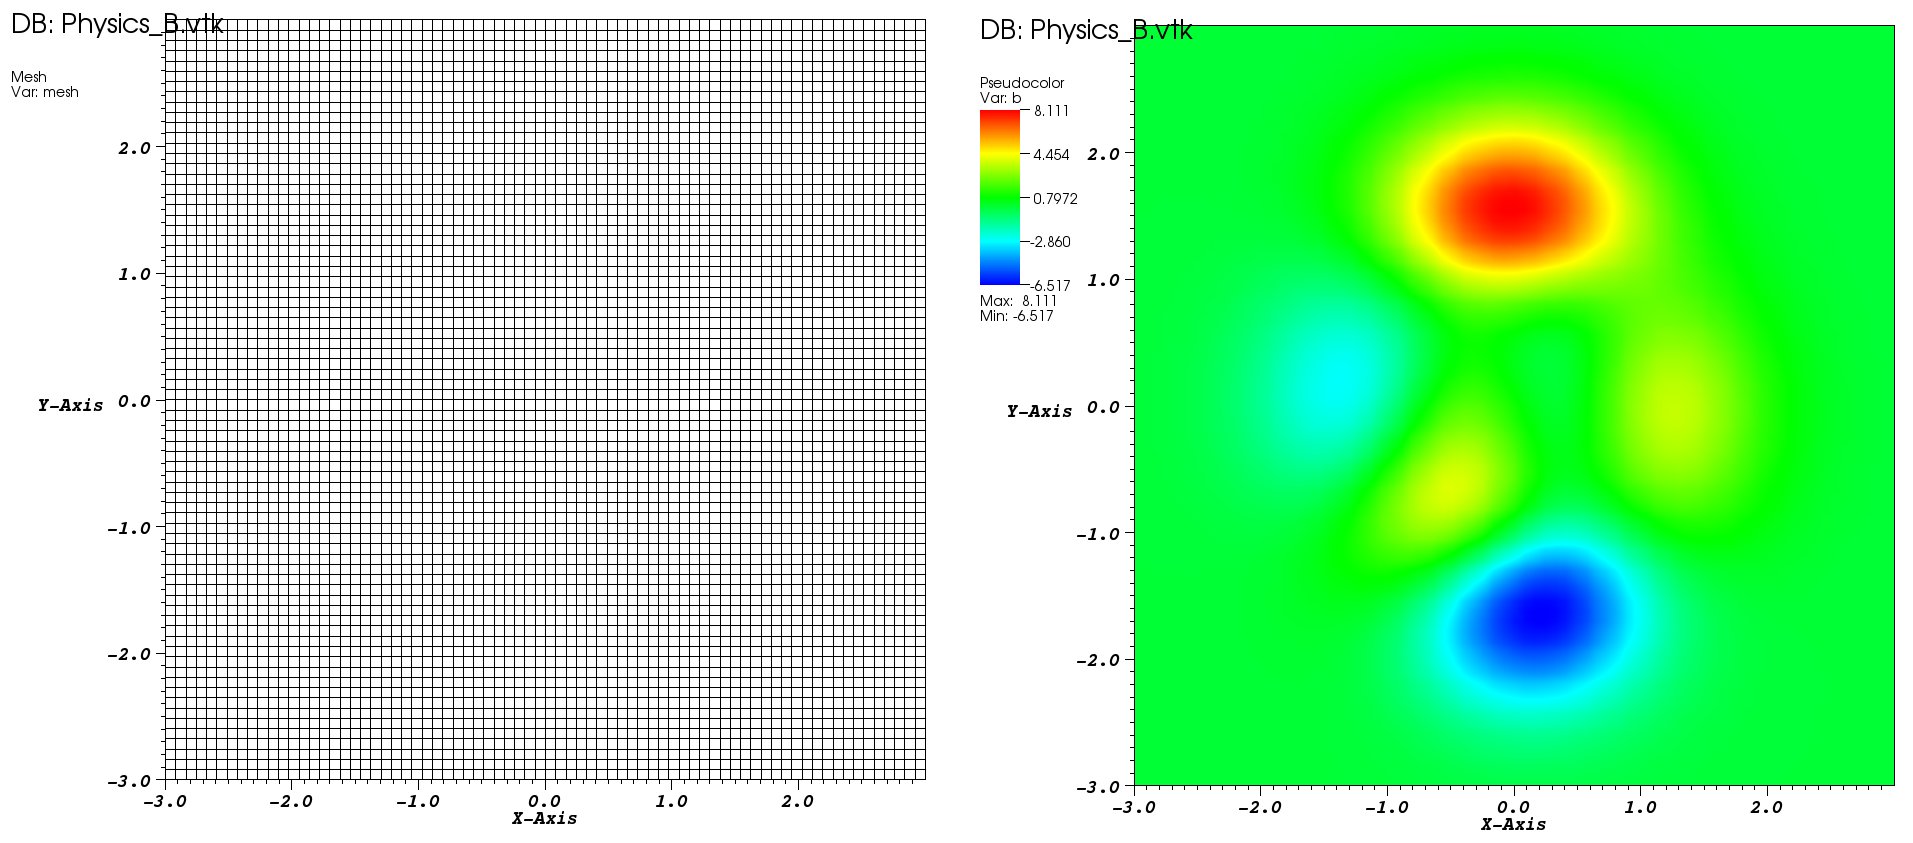
\includegraphics[width=6in]{images/sol_B.png}
  \end{center}
  \caption{\small \sl Coarse quad mesh (left) and peaks
    function solution (right) transferred to the code B mesh
    vertices.}
  \label{fig:sol_B}
\end{figure}

\section{Future Work}
It should be noted here that this example performed serial data
transfer. Furthermore, the transfer evaluator interface at present is
specifically defined for point coupling, both requesting from and
querying meshes for cartesian point coordinates. Future efforts should
include generalizing this package to operate on multiple forms of mesh
objects per the listed design requirements.

In addition to this, most other design requirements have not been
fulfilled. However, many of these requirements may be met by moving
the data structures, communication patterns, and algorithms already
existing in the coupler under the Denovo framework.

\appendix
\section{Transfer\_Evaluator Interface}
\begin{lstlisting}
//----------------------------------*-C++-*----------------------------------//
/*!
 * \file   core/Transfer_Evaluator.hh
 * \author Stuart Slattery
 * \date   Wed Oct 05 11:02:59 2011
 * \brief  Transfer_Evaluator class definition.
 */
//---------------------------------------------------------------------------//
// $Id: template.hh,v 1.4 2008/01/02 17:18:47 9te Exp $
//---------------------------------------------------------------------------//

#ifndef coupler_Transfer_Evaluator_hh
#define coupler_Transfer_Evaluator_hh

#include "comm/global.hh"
#include <vector>
#include <string>

namespace coupler
{

//===========================================================================//
/*!
 * \class Transfer_Evaluator
 * \brief Base class definition of the transfer evaluator interface.
 *
 * This interface is templated on the type of field data being
 * transfered. Handle type is fixed to integer and coordinate type is fixed to
 * double. These could be templated in the future.
 */
//===========================================================================//
template<class FieldType_T>
class Transfer_Evaluator 
{
  public:

    //@{
    //! Useful typedefs.
    typedef FieldType_T                              FieldType;
    typedef nemesis::Communicator_t                  Communicator;
    typedef int                                      Handle;
    typedef const Handle*                            Handle_Iterator;
    typedef double                                   Coordinate;
    typedef const Coordinate*                        Coord_Iterator;
    //@}

    //! Constructor.
    Transfer_Evaluator()
    { /* ... */ }

    //! Destructor.
    virtual ~Transfer_Evaluator()
    { /* ... */ }

    //! Register communicator object.
    virtual void register_comm(Communicator &comm) = 0;

    //! Register a field associated with the entities. Return false if this
    //! field is not supported.
    virtual bool register_field(std::string field_name) = 0;

    //! Register cartesian coordinates with a field. The coordinate vector
    //! should be interleaved. The handle vector should consist of globally
    //! unique handles. These iterators imply contiguous memory storage.
    virtual void register_xyz(std::string field_name,
			      Coord_Iterator &points_begin,
			      Coord_Iterator &points_end,
			      Handle_Iterator &handles_begin,
			      Handle_Iterator &handles_end) = 0;

    //! Given (x,y,z) coordinates and an associated globally unique handle,
    //! return true if in the local domain, false if not.
    virtual bool find_xyz(Coordinate x, 
			  Coordinate y,
			  Coordinate z,
			  Handle handle) = 0;

    //! Given an entity handle, get the field data associated with that
    //! handle.
    virtual void pull_data(std::string field_name,
			   Handle handle,
			   FieldType &data) = 0;

    //! Given an entity handle, set the field data associated with that
    //! handle.
    virtual void push_data(std::string field_name,
			   Handle handle, 
			   FieldType data) = 0;

    //! Perfom a global integration on a field for rebalance.
    virtual void integrate(std::string field_name,
			   FieldType &field_norm) = 0;

    //! Perform a rebalance on a field for conservation.
    virtual void rebalance(std::string field_name,
			   FieldType field_norm) = 0;
};

} // end namespace coupler

#endif // coupler_Transfer_Evaluator_hh

//---------------------------------------------------------------------------//
//              end of core/Transfer_Evaluator.hh
//---------------------------------------------------------------------------//
\end{lstlisting}

\section{Simple Example Listings}

\begin{lstlisting}
//----------------------------------*-C++-*----------------------------------//
/*!
 * \file   peaks_example/TE_Physics_A.cc
 * \author Stuart Slattery 
 * \date   Wed Oct 05 10:57:30 2011
 * \brief  Transfer Evaluator for Physics_A.
 */
//---------------------------------------------------------------------------//
// $Id: template.cc,v 1.3 2008/01/02 17:18:47 9te Exp $
//---------------------------------------------------------------------------//

#include "TE_Physics_A.hh"

namespace peaks_example
{
//---------------------------------------------------------------------------//
// Constructor.
TE_Physics_A::TE_Physics_A(physics_A::Physics_A* a_)
    : a(a_)
{ /* ... */ }

//---------------------------------------------------------------------------//
// Destructor.
TE_Physics_A::~TE_Physics_A()
{ /* ... */ }

//---------------------------------------------------------------------------//
//! Register a field associated with the entities.
bool TE_Physics_A::register_field(std::string field_name)
{
    if (field_name == "PEAKS") return true;
    else return false;
}

//---------------------------------------------------------------------------//
// Given (x,y,z) coordinates and an associated globally unique handle,
// return true if in the local domain, false if not.
bool TE_Physics_A::find_xyz(double x, 
			    double y, 
			    double z,
			    Handle handle)
{
    return a->get_xy_info(x, y, handle);
}

//---------------------------------------------------------------------------//
// Given an entity handle, get the field data associated with that handle.
void TE_Physics_A::pull_data(std::string field_name,
			     Handle handle,
			     double &data)
{
    if (field_name == "PEAKS")
    {
	a->get_state(handle, data);
    }
}

//---------------------------------------------------------------------------//

} // end namespace peaks_example

//---------------------------------------------------------------------------//
//                 end of TE_Physics_A.cc
//---------------------------------------------------------------------------//
\end{lstlisting}

\begin{lstlisting}
//----------------------------------*-C++-*----------------------------------//
/*!
 * \file   peaks_example/TE_Physics_B.cc
 * \author Stuart Slattery
 * \date   Wed Oct 05 10:57:33 2011
 * \brief  Transfer Evaluator for Physics_B.
 */
//---------------------------------------------------------------------------//
// $Id: template.cc,v 1.3 2008/01/02 17:18:47 9te Exp $
//---------------------------------------------------------------------------//

#include "TE_Physics_B.hh"

namespace peaks_example
{

//---------------------------------------------------------------------------//
// Constructor.
TE_Physics_B::TE_Physics_B(physics_B::Physics_B* b_)
    : b(b_)
{ /* ... */ }

//---------------------------------------------------------------------------//
// Destructor.
TE_Physics_B::~TE_Physics_B()
{ /* ... */ }

//---------------------------------------------------------------------------//
//! Register a field associated with the entities.
bool TE_Physics_B::register_field(std::string field_name)
{
    if (field_name == "PEAKS") return true;
    else return false;
}

//---------------------------------------------------------------------------//
// Register cartesian coordinates with a field. The coordinate vector
// should be interleaved. The handle vector should consist of globally
// unique handles. These iterators imply contiguous memory storage.
void TE_Physics_B::register_xyz(std::string field_name,
				Coord_Iterator &points_begin,
				Coord_Iterator &points_end,
				Handle_Iterator &handles_begin,
				Handle_Iterator &handles_end)
{
    if (field_name == "PEAKS")
    {
	// Vector setup.
	points.resize( 3*(b->x_domain().size())*(b->y_domain().size()) );
	handles.resize( points.size() / 3 );

	// Set iterators.
	Coord_Iterator x_it;
	Coord_Iterator y_it;
	Coord_Iterator coord_it = points.begin();
	Handle_Iterator handle_it = handles.begin();

	// Populate the coordinate and handle vectors.
	int handle_counter = 0;
	for (y_it = b->y_domain().begin(); 
	     y_it != b->y_domain().end(); 
	     ++y_it)
	{
	    for (x_it = b->x_domain().begin(); 
		 x_it != b->x_domain().end(); 
		 ++x_it)
	    {
		*coord_it = *x_it;
		++coord_it;

		*coord_it = *y_it;
		++coord_it;

		*coord_it = 0.0;
		++coord_it;

		*handle_it = handle_counter;
		++handle_it;
		++handle_counter;
	    }
	}

	// Return the iterators.
	points_begin = points.begin();
	points_end = points.end();
	handles_begin = handles.begin();
	handles_end = handles.end();
    }
}

//---------------------------------------------------------------------------//
// Push data onto a field.
void TE_Physics_B::push_data(std::string field_name,
			     Handle handle, 
			     double data)
{
    b->set_source(handle, data);
}

//---------------------------------------------------------------------------//

} // end namespace peaks_example

//---------------------------------------------------------------------------//
//                 end of TE_Physics_B.cc
//---------------------------------------------------------------------------//
\end{lstlisting}

\pagebreak
\bibliographystyle{ieeetr}
\bibliography{paper}
\end{document}


